\section{Results}
\label{sec:results}
\subsection{Discrimination across three training seeds}
All 45 principal-model runs and 15 supplementary mean-pooling runs completed training and formal evaluation. Sixty evaluation receipts and 180 registered report identities were verified. Every seed-specific predictor averaged five fold probabilities for each of the same 175 holdout patients, including 56 positive outcomes. We then calculated metrics within each seed and averaged the metrics across seeds 42, 44, and 2026. Table~\ref{tab:main} reports means with sample seed standard deviations; conditional patient intervals and paired tests are reported separately.
\begin{table*}[t]
\centering
\small
\caption{Performance on the fixed internal holdout (175 patients, 56 pCR positive). Entries are mean $\pm$ sample SD over seeds 42, 44, and 2026. Within each seed, five fold probabilities are averaged per patient before metrics; no probabilities are averaged across seeds. Macro averages T0--T2 metrics within each seed. F1 uses threshold 0.5. Paired Macro differences and adjusted tests are in Table~\ref{tab:bootstrap}.}
\label{tab:main}
\begin{tabular}{llrrr}
\toprule
Model & Landmark & AUROC & AP & F1 \\
\midrule
NoJEPA & T0 & 0.7261 $\pm$ 0.0039 & 0.5944 $\pm$ 0.0010 & 0.5370 $\pm$ 0.0161 \\
NoJEPA & T1 & 0.7234 $\pm$ 0.0054 & 0.5956 $\pm$ 0.0031 & 0.5421 $\pm$ 0.0120 \\
NoJEPA & T2 & 0.7234 $\pm$ 0.0041 & 0.5941 $\pm$ 0.0041 & 0.5484 $\pm$ 0.0115 \\
NoJEPA & Macro & 0.7243 $\pm$ 0.0040 & 0.5947 $\pm$ 0.0027 & 0.5425 $\pm$ 0.0132 \\
DirectReadout & T0 & 0.7344 $\pm$ 0.0109 & 0.5966 $\pm$ 0.0075 & 0.5412 $\pm$ 0.0226 \\
DirectReadout & T1 & 0.7364 $\pm$ 0.0130 & 0.6077 $\pm$ 0.0069 & 0.5421 $\pm$ 0.0309 \\
DirectReadout & T2 & 0.7350 $\pm$ 0.0086 & 0.6023 $\pm$ 0.0095 & 0.5580 $\pm$ 0.0103 \\
DirectReadout & Macro & 0.7353 $\pm$ 0.0107 & 0.6022 $\pm$ 0.0052 & 0.5471 $\pm$ 0.0206 \\
ForecastAttention & T0 & 0.7437 $\pm$ 0.0025 & 0.6166 $\pm$ 0.0079 & 0.5547 $\pm$ 0.0185 \\
ForecastAttention & T1 & 0.7460 $\pm$ 0.0053 & 0.6170 $\pm$ 0.0101 & 0.5507 $\pm$ 0.0141 \\
ForecastAttention & T2 & 0.7464 $\pm$ 0.0074 & 0.6170 $\pm$ 0.0127 & 0.5615 $\pm$ 0.0197 \\
ForecastAttention & Macro & 0.7454 $\pm$ 0.0047 & 0.6169 $\pm$ 0.0102 & 0.5556 $\pm$ 0.0143 \\
\bottomrule
\end{tabular}
\end{table*}


\fullmodel{} had mean T0/T1/T2 AUROCs of 0.7437/0.7460/0.7464 and AP values of 0.6166/0.6170/0.6170 (Fig.~\ref{fig:discrimination}). Its Macro AUROC/AP/F1 was 0.7454/0.6169/0.5556, with seed standard deviations of 0.0047/0.0102/0.0143. Corresponding means were 0.7243/0.5947/0.5425 for \nojepa{} and 0.7353/0.6022/0.5471 for \direct{}. The full model therefore had the highest mean AUROC and AP at every landmark among the three principal variants and the highest mean Macro F1. Its T2 F1 was 0.5615, compared with 0.5580 for \direct{} and 0.5484 for \nojepa{}.

\begin{figure*}[t]
\centering
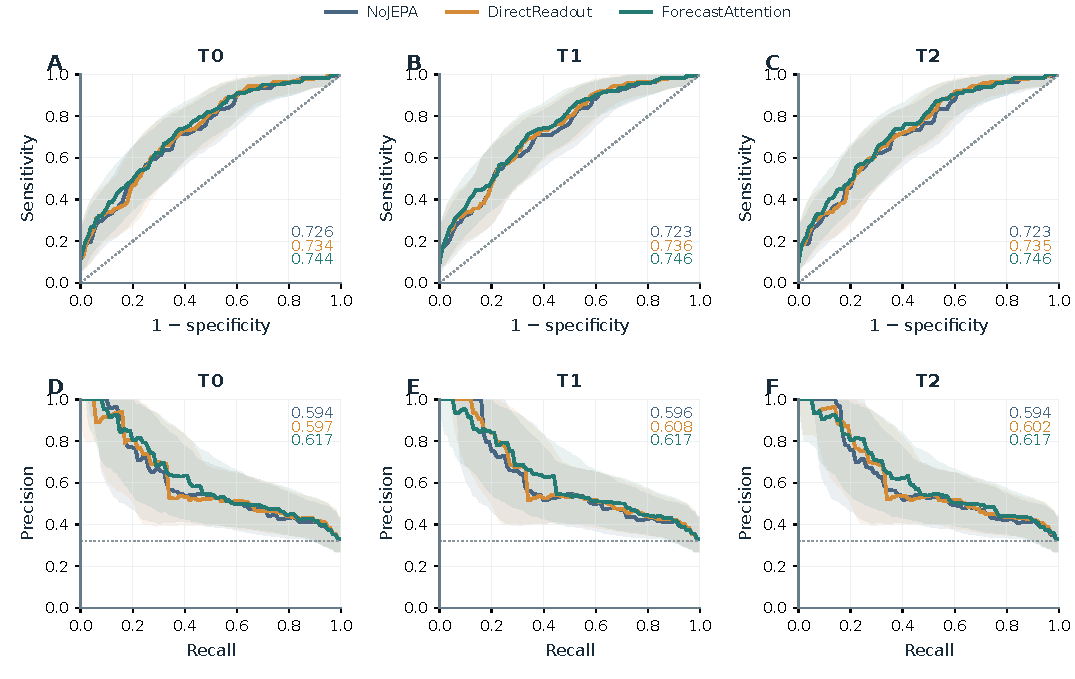
\includegraphics[width=\textwidth]{figures/discrimination.pdf}
\caption{Discrimination across seeds 42, 44, and 2026. (A--C) Mean ROC curves; (D--F) mean precision--recall curves. Curves are computed from five-fold ensemble probabilities separately within each seed, interpolated on a common grid, and equally averaged across seeds. Shading gives pointwise conditional 95\% shared-patient-bootstrap intervals for the mean curve. Colored metric values are means of the directly computed seed-specific AUROC or non-interpolated AP; they need not equal the area under the displayed mean curve. The dotted PR reference is the 0.32 positive prevalence.}
\label{fig:discrimination}
\end{figure*}

Under direct readout, adding future-state supervision increased mean Macro AUROC/AP/F1 by +0.0110/+0.0075/+0.0046. The complete forecast-attention readout gave further mean increases of +0.0101/+0.0147/+0.0085 relative to \direct{}. These mean differences conceal variation among the seeds. The direct-versus-\nojepa{} Macro AUROC difference was positive at seeds 42 and 44 but negative at seed 2026 (0.7230 versus 0.7251). Likewise, \fullmodel{} exceeded \direct{} in Macro AUROC at seeds 44 and 2026 but was slightly lower at seed 42 (0.7419 versus 0.7428). The full-versus-\nojepa{} Macro AUROC difference was positive at all three selected seeds. Individual results are retained in Table~\ref{tab:seedresults}; the subset does not establish uniform behavior across all possible seeds.

The supplementary \meanmodel{} had mean Macro AUROC/AP/F1 of 0.7454/0.6132/0.5723 (Table~\ref{tab:pooling}). Its Macro AUROC was exactly equal to the attention model's at the available numerical precision, while its mean F1 was higher. Attention had a higher AP point estimate, but the mean-pooling control had the highest mean Macro F1 among all four variants. This comparison provides no uniform attention advantage.

Paired patient intervals qualify the descriptive rankings (Fig.~\ref{fig:paired}). The mean Macro AUROC difference for \fullmodel{} versus \nojepa{} was +0.0211 [0.0090, 0.0345]. The corresponding \direct{}--\nojepa{} difference was +0.0110 [$-0.0021$, 0.0243], and the \fullmodel{}--\direct{} difference was +0.0101 [$-0.0047$, 0.0255]. The full-versus-\nojepa{} AP difference was +0.0222 [0.0017, 0.0451], whereas its F1 difference was +0.0131 [$-0.0086$, 0.0381]. All three full-versus-direct Macro intervals included zero. These intervals concern patient sampling conditional on the selected fitted predictors and are distinct from the descriptive seed standard deviations.
The full-versus-\nojepa{} Macro AUROC difference had an approximate paired-bootstrap raw $p=0.00224$ and $p_{\mathrm{Holm}}=0.02016$ within the nine-comparison principal family. It was the only principal comparison below the family-adjusted 0.05 criterion. Its adjusted value increased to 0.19488 when all 90 reported tests were considered together. The AP comparison had raw/within-family adjusted $p=0.04344/0.34752$, and the full-versus-direct AUROC comparison had 0.18461/1.0000. Thus the support for the complete-versus-control AUROC difference depends on the reporting family and remains exploratory. Nonsignificant comparisons do not establish equivalence.
\begin{table*}[t]
\centering
\small
\caption{Exploratory principal Macro comparisons. All metrics use approximate, null-centered paired patient-bootstrap tests with 99,999 shared resamples. Within each draw, metrics are computed for each seed then equally averaged. All $p$ values are two-sided. Holm$_9$ adjusts the nine entries here; Holm$_{90}$ is the sensitivity analysis over all principal and secondary tests. Sig. refers to Holm$_9$. Direct and Attention abbreviate DirectReadout and ForecastAttention. $^{*}p_{\mathrm{Holm}}<0.05$, $^{**}p_{\mathrm{Holm}}<0.01$, $^{***}p_{\mathrm{Holm}}<0.001$; ns, not significant after the stated correction. Intervals are unadjusted 95\% patient-bootstrap intervals (2,000 shared draws) and need not agree with adjusted test decisions. All analyses condition on the fixed, retrospectively selected seed42/44/2026 ensembles; seeds are not resampled.}
\label{tab:bootstrap}
\begin{tabular}{llrrrrc}
\toprule
Comparison & Metric & Difference [95\% CI] & $p$ & $p_{\mathrm{Holm},9}$ & $p_{\mathrm{Holm},90}$ & Sig. \\
\midrule
Direct -- NoJEPA & AUROC & +0.0110 [-0.0021, +0.0243] & 0.0958 & 0.6705 & 1.0000 & ns \\
Direct -- NoJEPA & AP & +0.0075 [-0.0079, +0.0251] & 0.3588 & 1.0000 & 1.0000 & ns \\
Direct -- NoJEPA & F1 & +0.0046 [-0.0165, +0.0233] & 0.6354 & 1.0000 & 1.0000 & ns \\
Attention -- NoJEPA & AUROC & +0.0211 [+0.0090, +0.0345] & 0.0022 & 0.0202 & 0.1949 & * \\
Attention -- NoJEPA & AP & +0.0222 [+0.0017, +0.0451] & 0.0434 & 0.3475 & 1.0000 & ns \\
Attention -- NoJEPA & F1 & +0.0131 [-0.0086, +0.0381] & 0.2786 & 1.0000 & 1.0000 & ns \\
Attention -- Direct & AUROC & +0.0101 [-0.0047, +0.0255] & 0.1846 & 1.0000 & 1.0000 & ns \\
Attention -- Direct & AP & +0.0147 [-0.0058, +0.0366] & 0.1711 & 1.0000 & 1.0000 & ns \\
Attention -- Direct & F1 & +0.0085 [-0.0178, +0.0389] & 0.5456 & 1.0000 & 1.0000 & ns \\
\bottomrule
\end{tabular}
\end{table*}


\begin{figure*}[t]
\centering
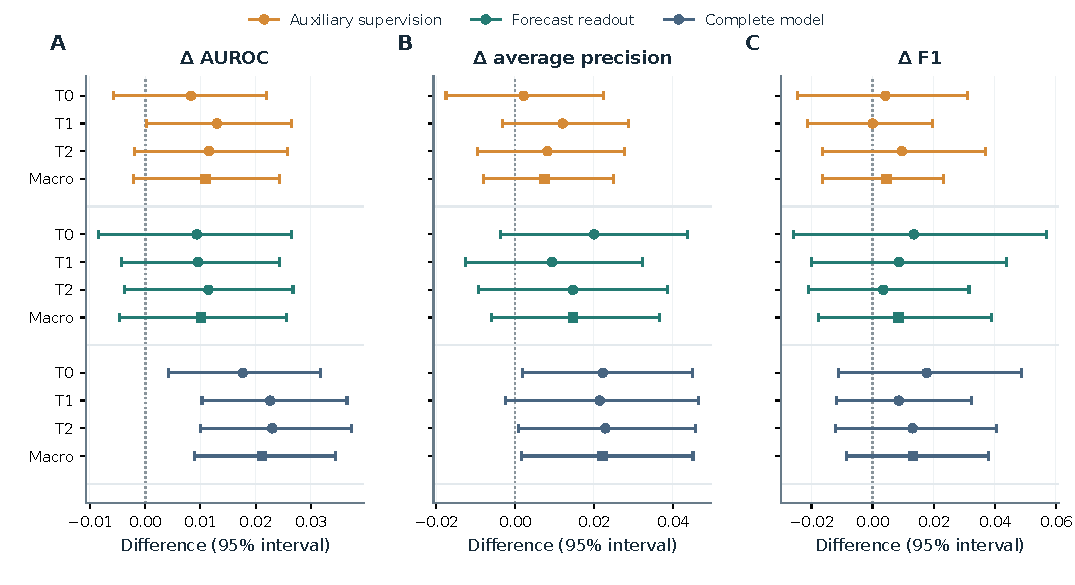
\includegraphics[width=\textwidth]{figures/paired_comparisons.pdf}
\caption{Paired seed-mean metric differences at T0, T1, T2, and Macro. Colors distinguish auxiliary supervision, additional forecast readout, and the complete-model contrast. Squares denote Macro estimates. Bars are unadjusted 95\% patient-bootstrap intervals. Every draw is shared across seeds, models, and landmarks; metrics are computed within seed before averaging. Adjusted tests appear in Tables~\ref{tab:bootstrap} and~\ref{tab:significance_landmarks}. Folds, seeds, and repeated landmarks do not create independent test cohorts.}
\label{fig:paired}
\end{figure*}

\subsection{Threshold behavior and class imbalance}
\begin{table*}[t]
\centering
\small
\caption{Operating characteristics at threshold 0.5. Entries average the three seed-specific fivefold probability-ensemble metrics; Macro first averages T0--T2 within each seed. The same 175 patients appear in every evaluation.}
\label{tab:extended_operating}
\begin{tabular}{llrrrrrr}
\toprule
Model & Landmark & Sens. & Spec. & PPV & NPV & BA & MCC \\
\midrule
NoJEPA & T0 & 0.595 & 0.709 & 0.491 & 0.789 & 0.652 & 0.292 \\
NoJEPA & T1 & 0.607 & 0.703 & 0.491 & 0.792 & 0.655 & 0.297 \\
NoJEPA & T2 & 0.619 & 0.700 & 0.494 & 0.797 & 0.660 & 0.304 \\
NoJEPA & Macro & 0.607 & 0.704 & 0.492 & 0.793 & 0.656 & 0.298 \\
\midrule
DirectReadout & T0 & 0.577 & 0.739 & 0.513 & 0.789 & 0.658 & 0.309 \\
DirectReadout & T1 & 0.583 & 0.734 & 0.509 & 0.790 & 0.659 & 0.308 \\
DirectReadout & T2 & 0.643 & 0.689 & 0.494 & 0.804 & 0.666 & 0.314 \\
DirectReadout & Macro & 0.601 & 0.721 & 0.505 & 0.794 & 0.661 & 0.310 \\
\midrule
ForecastAttention & T0 & 0.631 & 0.697 & 0.495 & 0.801 & 0.664 & 0.312 \\
ForecastAttention & T1 & 0.649 & 0.667 & 0.482 & 0.802 & 0.658 & 0.299 \\
ForecastAttention & T2 & 0.661 & 0.675 & 0.491 & 0.810 & 0.668 & 0.318 \\
ForecastAttention & Macro & 0.647 & 0.680 & 0.489 & 0.804 & 0.663 & 0.310 \\
\bottomrule
\end{tabular}
\end{table*}

At threshold 0.5, mean Macro sensitivity/NPV was 0.6468/0.8042 for \fullmodel{}, compared with 0.6012/0.7943 for \direct{}. These increases accompanied lower specificity (0.6797 versus 0.7208) and PPV (0.4894 versus 0.5053). The paired mean sensitivity difference was +0.0456 [0.0099, 0.0866], while the specificity difference was $-0.0411$ [$-0.0649$, $-0.0202$]. These unadjusted intervals describe an operating trade-off rather than a general classification improvement. The specificity decrease had raw $p=0.00048$, secondary-family Holm $p=0.03888$, and all-90 Holm $p=0.04320$. It was the only secondary comparison meeting its family-adjusted 0.05 criterion; the sensitivity increase did not ($p_{\mathrm{Holm}}=1.0000$).

The independent 999,999-resample Monte Carlo stability check gave specificity $p=0.000434$ (simulation standard error 0.0000208). Holding the other 89 values fixed yielded secondary-family and all-90 adjusted values of 0.035154 and 0.03906, respectively, preserving the adverse-specificity conclusion. The main tables retain the uniformly generated 99,999-resample values.

The full model's seed-mean true-positive counts at T0/T1/T2 were 35.33/36.33/37.00, with false-positive counts 36.00/39.67/38.67. These are averages of integer counts from three correlated predictors, not fractional patients or a single combined confusion matrix. T1 added positive predictions while mean F1 decreased from 0.5547 at T0 to 0.5507; T2 F1 then increased to 0.5615. Later information can change error balance differently from ranking.

Among the principal variants, \fullmodel{} had the highest mean Macro balanced accuracy (0.6633), while \direct{} had slightly higher MCC (0.3105 versus 0.3096) and accuracy (0.6825 versus 0.6692). \nojepa{} had balanced accuracy 0.6556, MCC 0.2976, and accuracy 0.6730. The all-negative accuracy reference is 0.68 in this cohort: direct readout marginally exceeded it, whereas the other principal variants did not. The supplementary \meanmodel{} reached balanced accuracy 0.6774, MCC 0.3349, and accuracy 0.6813. Accuracy, ranking, and class-specific errors therefore give different descriptive orderings.

OOF-selected Youden thresholds changed mean holdout Macro F1 from 0.5425 to 0.5472 for \nojepa{}, 0.5471 to 0.5434 for \direct{}, 0.5556 to 0.5537 for \fullmodel{}, and 0.5723 to 0.5666 for \meanmodel{} (Table~\ref{tab:extended_threshold}). Thus the alternative threshold did not consistently improve F1. These results concern transfer of thresholds fitted on single-model OOF scores to within-seed five-model ensemble scores; they neither optimize a holdout threshold nor establish independent ensemble calibration.

\subsection{Longitudinal information and probability quality}
The paired seed-mean T2--T0 AUROC change was +0.0027 [$-0.0030$, 0.0089] for \fullmodel{}, $-0.0027$ [$-0.0085$, 0.0027] for \nojepa{}, and +0.0006 [$-0.0045$, 0.0054] for \direct{}. The full model's corresponding AP change was +0.0004 [$-0.0099$, 0.0113] and F1 change +0.0068 [$-0.0101$, 0.0253]. All these longitudinal intervals included zero. The increasing mean AUROC for forecast attention across landmarks therefore remains a small descriptive trend. Fig.~\ref{fig:scorechanges} shows outcome-conditioned distributions of changes in seed-specific ensemble probabilities.

\begin{table*}[t]
\centering
\small
\caption{Probability quality: three-seed mean $\pm$ sample SD of Macro metrics. Each seed has its own fivefold probability ensemble. Lower is better; ECE uses ten equal-width bins.}
\label{tab:calibration}
\begin{tabular}{lrrr}
\toprule
Model & NLL & Brier & ECE \\
\midrule
NoJEPA & 0.5839 $\pm$ 0.0074 & 0.2008 $\pm$ 0.0031 & 0.1193 $\pm$ 0.0223 \\
DirectReadout & 0.5763 $\pm$ 0.0126 & 0.1977 $\pm$ 0.0055 & 0.1215 $\pm$ 0.0249 \\
ForecastAttention & 0.5823 $\pm$ 0.0146 & 0.1998 $\pm$ 0.0055 & 0.1348 $\pm$ 0.0296 \\
\bottomrule
\end{tabular}
\end{table*}

Mean Macro NLL/Brier/ECE was 0.5823/0.1998/0.1348 for \fullmodel{}, compared with 0.5763/0.1977/0.1215 for \direct{} and 0.5839/0.2008/0.1193 for \nojepa{}. Forecast attention had worse point estimates of all three probability-quality metrics than direct readout. Against \nojepa{}, it had slightly better NLL and Brier score but higher ECE; these metrics did not support a single calibration ordering. All 14 Macro metrics and their conditional patient intervals appear in Table~\ref{tab:extended_macro}.

\begin{figure*}[t]
\centering
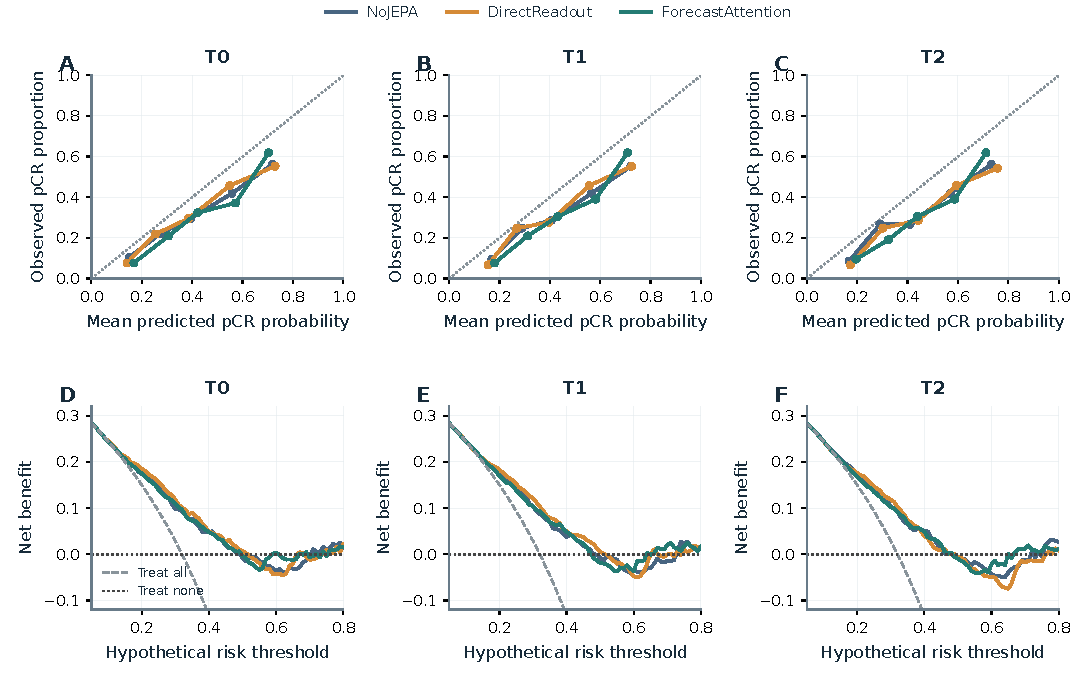
\includegraphics[width=\textwidth]{figures/calibration_utility.pdf}
\caption{Probability quality and hypothetical decision utility across three seeds. (A--C) Reliability summaries first form five equal-count probability-rank groups of 35 patients within each seed-specific five-fold ensemble and then average the group summaries across seeds. They differ from the ten equal-width bins used for ECE. (D--F) Net-benefit curves are computed separately within seeds and then averaged, with treat-all and treat-none references. Scores are not recalibrated. No clinical escalation or de-escalation strategy is validated.}
\label{fig:calutility}
\end{figure*}

\subsection{Hypothetical net benefit}
Decision curves did not preserve the discrimination ranking across thresholds. At a hypothetical threshold of 0.30, mean Macro net benefit was 0.1192 for \direct{} and 0.1050 for \fullmodel{}. At 0.50, it was $-0.0070$ for \nojepa{}, +0.0025 for \direct{}, and $-0.0108$ for \fullmodel{}. At 0.70 the ordering reversed, with +0.0089 for \fullmodel{} and $-0.0104$ for \direct{}. These values average seed-specific decision curves, use uncalibrated probabilities, and assume a generic positive action. They do not establish an acceptable clinical threshold or validate a management pathway.

\subsection{Exploratory biological and acquisition-related subgroups}
The four HR/HER2 groups had positive seed-mean Macro AUROC differences between \fullmodel{} and \nojepa{} (Fig.~\ref{fig:subgroups}; Table~\ref{tab:subgroups}). The HR-positive/HER2-negative group had a difference of +0.0333 [0.0072, 0.0653] among 68 patients, including 11 positive outcomes. Other differences were +0.0171 [$-0.0466$, 0.0864] in HR-positive/HER2-positive patients (31, 12 positive), +0.0363 [$-0.0408$, 0.1474] in HR-negative/HER2-positive patients (14, 7 positive), and +0.0224 [$-0.0060$, 0.0551] in HR-negative/HER2-negative patients (62, 26 positive). Only the first subgroup's unadjusted interval excluded zero. These intervals were not multiplicity-adjusted and do not establish an interaction or a confirmed subtype-specific benefit.

In the HR-positive/HER2-negative group, forecast attention's mean Macro sensitivity/specificity was 0.1414/0.9766, compared with 0.1212/0.9825 for \nojepa{}. Thus low sensitivity at threshold 0.5 persisted despite the positive AUROC difference. \direct{} had sensitivity/specificity 0.1010/0.9883 and a slightly higher mean AUROC than forecast attention (0.7108 versus 0.7087). The age groups also had positive full-versus-control differences, but their unadjusted exploratory intervals do not support an age-interaction conclusion. Source namespaces share one clinical release and do not constitute external validation. The partially clipped baseline-component group contained only 11 patients and one positive outcome; its AUROC and AP were suppressed under the minimum-outcome rule.

\begin{figure*}[t]
\centering
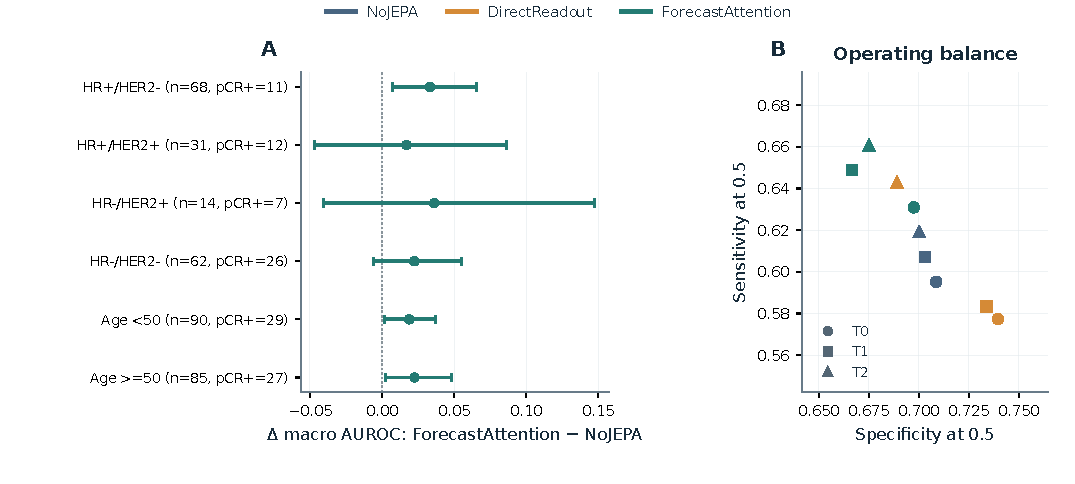
\includegraphics[width=\textwidth]{figures/subgroup_operating.pdf}
\caption{Exploratory subgroup and operating-point summaries, with metrics computed within seed and then equally averaged across seeds 42, 44, and 2026. (A) Macro AUROC differences between ForecastAttention and NoJEPA within HR/HER2 and age groups, with patient counts, positive outcomes, and unadjusted shared-patient intervals. No subgroup-interaction claim is made. (B) Mean specificity and sensitivity at threshold 0.5 across landmarks; colors identify models and markers identify landmarks.}
\label{fig:subgroups}
\end{figure*}

\subsection{Archived forecast and gradient diagnostics}
Archived fixed-training-probe diagnostics describe individual models separately from the pCR holdout analysis (Fig.~\ref{fig:mechanism}). At common epoch 20, mean copy-normalized forecast skills for \direct{} were +0.0068, +0.0551, and +0.1724 at one-, two-, and three-step horizons. Corresponding values for \fullmodel{} were $-0.0576$, $-0.0584$, and +0.0089 (Table~\ref{tab:worldprobe}). Statistics were normalized within each snapshot's EMA coordinates, averaged across five folds within seed, and then averaged across the three seeds. Separate models' latent states were not ensembled. These diagnostics do not support attributing forecast attention's pCR ranking to uniformly more accurate latent forecasts.

The probe requires the real landmark, target, and every intermediate examination, whereas the training objective masks unavailable future targets. Eligible populations therefore vary by horizon; only 5--9 patients per probe were eligible at three steps. These measurements are not selected-checkpoint holdout forecast evaluations. The predictor's pCR-loss gradient norm was zero for \direct{} and had mean 1.0033 for \fullmodel{}; weighted rollout-gradient means were 0.1482 and 0.1673. These values support the expected gradient routing, but gradient magnitude is not a biological effect size. \nojepa{} had no available trained-world diagnostic and was not assigned an artificial zero skill.

\begin{figure*}[t]
\centering
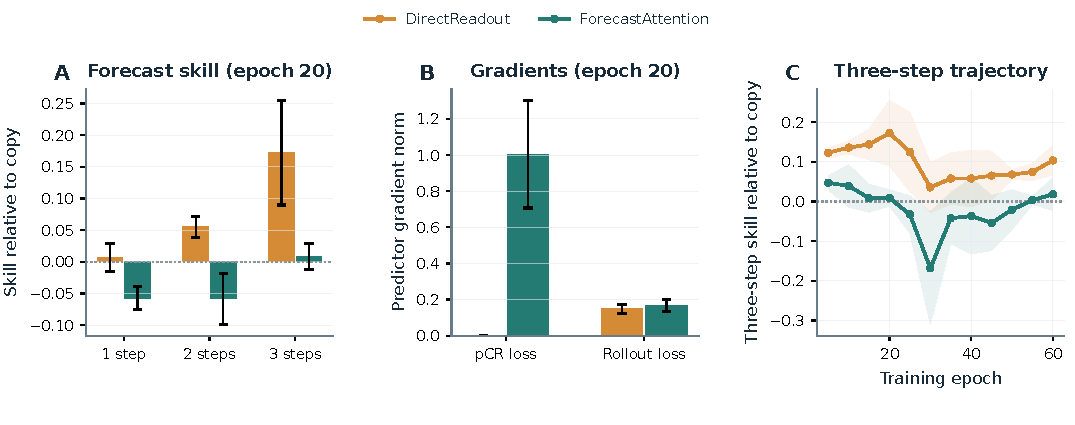
\includegraphics[width=\textwidth]{figures/forecast_mechanism.pdf}
\caption{Archived fixed-training-probe diagnostics across three seeds. (A) Copy-normalized forecast skill at common epoch 20. (B) Predictor gradient norms from pCR and weighted rollout losses. (C) Three-step skill across epochs with complete diagnostic coverage. Statistics are calculated within each snapshot's EMA coordinates, averaged across folds within seed, and summarized across seeds. These are training diagnostics, distinct from pCR probability ensembling; real continuous visit chains are required, and three-step eligibility is only 5--9 patients per probe.}
\label{fig:mechanism}
\end{figure*}
